\documentclass[a4paper,12pt]{report}

\usepackage[unicode,colorlinks=true,linkcolor=blue]{hyperref}
% здесь подключении шрифтов в русскими буквами
\usepackage[T2A]{fontenc}
\usepackage[utf8]{inputenc}
\usepackage[english,russian]{babel}
\usepackage{amsmath,amsthm,amssymb,amsfonts,mathtext,cite,enumerate,float}
%\usepackage[dvips]{graphicx}
\usepackage[pdftex]{graphicx}
\graphicspath{{images/}}
\usepackage{fix-cm}

\makeatletter
\renewcommand{\@biblabel}[1]{#1.}
\makeatother

\usepackage{geometry}  % Меняем поля страницы
\geometry{left=2cm}    % левое поле
\geometry{right=1.5cm} % правое поле
\geometry{top=1cm}     % верхнее поле
\geometry{bottom=2cm}  % нижнее поле

\newcommand{\HRule}{\rule{\linewidth}{0.5mm}}

\renewcommand{\theenumi}{\arabic{enumi}}                                       % Меняем везде перечисления на цифра.цифра
\renewcommand{\labelenumi}{\arabic{enumi}}                                     % Меняем везде перечисления на цифра.цифра
\renewcommand{\theenumii}{.\arabic{enumii}}                                    % Меняем везде перечисления на цифра.цифра
\renewcommand{\labelenumii}{\arabic{enumi}.\arabic{enumii}.}                   % Меняем везде перечисления на цифра.цифра
\renewcommand{\theenumiii}{.\arabic{enumiii}}                                  % Меняем везде перечисления на цифра.цифра
\renewcommand{\labelenumiii}{\arabic{enumi}.\arabic{enumii}.\arabic{enumiii}.} % Меняем везде перечисления на цифра.цифра

\theoremstyle{plain}
\newtheorem{theorem}{Теорема}[section]
\newtheorem{lemma}[theorem]{Лемма}
\theoremstyle{definition}
\newtheorem{definition}{Определение}
\theoremstyle{remark}
\newtheorem*{example}{Пример}
\newtheorem*{remark}{Замечание}


\begin{document}
  % \begin{titlepage}
  \begin{center}
    Министерство общего и профессионального образования\\
    Российской Федерации \\[1em]

    НАЦИОНАЛЬНЫЙ ИССЛЕДОВАТЕЛЬСКИЙ ЯДЕРНЫЙ\\
    УНИВЕРСИТЕТ ``МИФИ'' \\[1em]

    \begin{minipage}{\textwidth}
      \begin{flushleft}
        \begin{tabular}{ l l }
          Факультет & Кибернетики и информационной безопасности\\
          Кафедра   & Информационные технологии в социальных системах
        \end{tabular}
      \end{flushleft}
    \end{minipage}\\[1em]

    \begin{minipage}{\textwidth}
      \begin{flushright}
        \textit{К защите допустить:}\\
        Заведующий кафедрой\\
        \underline{\hspace*{4.5cm}} М.\,В.~Сергиевский
      \end{flushright}
    \end{minipage}\\[3em]

    {ПОЯСНИТЕЛЬНАЯ ЗАПИСКА}\\
    {к курсовому проекту}\\
    {на тему:}\\[1em]
    \textbf{РАЗРАБОТКА АЛГОРИТМА ДЛЯ ВЫДЕЛЕНИЯ ЧАСТОВСТРЕЧАЮЩИХСЯ ШАБЛОНОВ
      ОШИБОК ИЗ ФАЙЛОВ ЖУРНАЛОВ ПРИЛОЖЕНИЙ}\\[1em]


    % {БГУИР ДП \textbf{1-31 03 04 07 093} ПЗ}\\[2em]
    \vfill

    \begin{tabular}{ p{0.65\textwidth}p{0.25\textwidth} }

      Студент: & А.\,Г.~Тропин \\

      \vfill
      Научный руководитель:\\
      к.т.н, доцент & М.\,В.~Сергиевский \\
      % Консультанты: &\\
      % \hspace*{3ex}\emph{от кафедры информатики} & А.\,А.~Волосевич \\
      % \hspace*{3ex}\emph{по экономической части} & А.\,В.~Рябов \\
      % \hspace*{3ex}\emph{по охране труда} & Е.\,А.~Колосова \\
      & \\
    \end{tabular}
    \vfill
    {\normalsize Москва 2015}
  \end{center}
\end{titlepage}






  Разработка алгоритма для выделения частовстречающихся шаблонов ошибок из log-файлов программ
  \tableofcontents

  \chapter*{Введение}
  \addcontentsline{toc}{chapter}{Введение}
  Большинство программных систем, имеющих сложную структуру и состоящих из нескольких сотен различных компонент(балансеры, верхние, средние метапоиски, промежуточные и базовые поиски, колдунщики, антироботы, свежесть, региональные поиск, несколько десятков параллельных поисков) обладают рядом схожих проблем. Напимер веб-поиск. Краткое схематичное описание архитектуры:

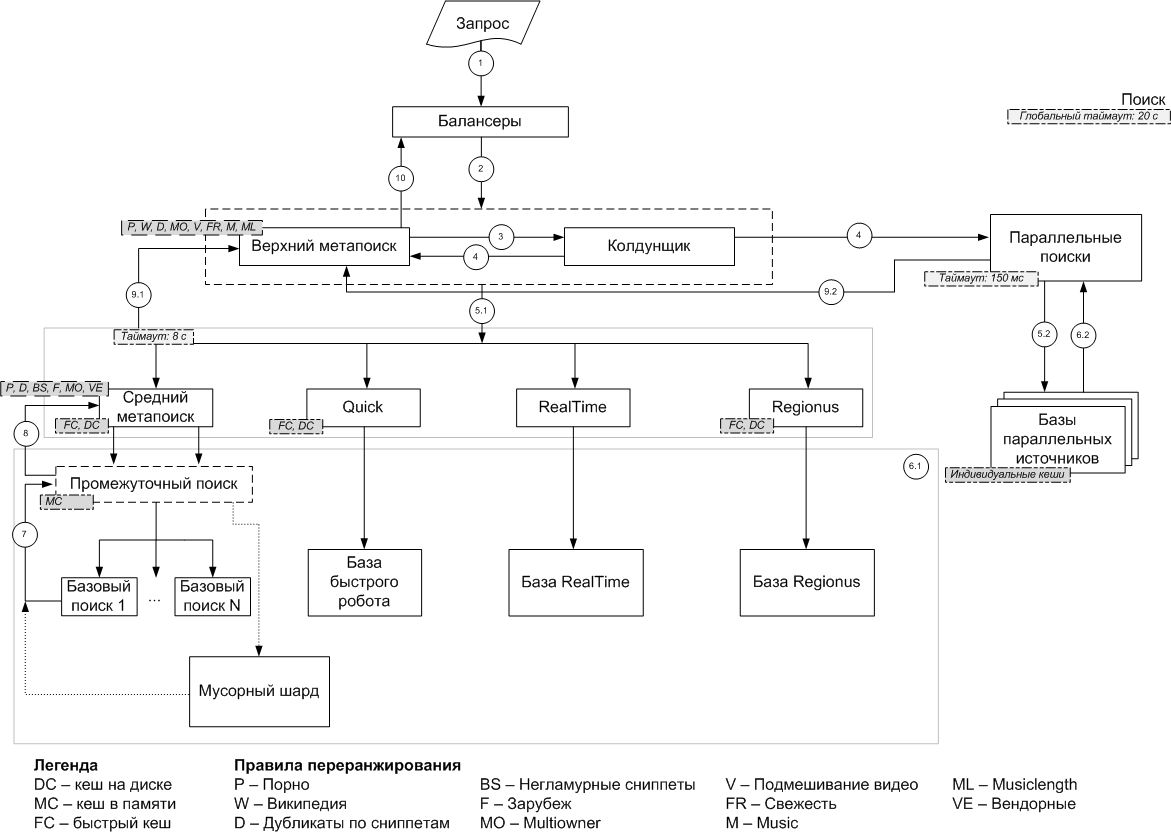
\includegraphics[width=\textwidth]{pics/search.png}

Всего единовременно запущено несколько ******** тысяч приложений. Каждое приложение генерирует множество ошибок и записывает каждую из них в log-файл.
Некоторые приложения, близкие по функционалу, пишут в один и тот же файл. Log-файлы ротируются согласно определённому алгоритму. Тем не менее объем log-файла для одного инстанса приложения может достигать нескольких сотен мегабайт, что препятствует быстрому ручному анализу в случае инцидента и инженеры вынуждены тратить ценные секунды на просмотр сотен тысяч строк файла в поисках сообщения с описанием элемента, вызвавшего сбой работы системы.

Начальным требованием к системе для эффективного использования алгоритма является наличие сопоставимого с количеством поисковых приложений количества нод на которых может быть запущена программа, реализующая алгоритм.

В организации, в которой выполнялась учебно-исследовательская работа, развернута большая поисковая инфраструктура, которая не лишена недостатков и существует вероятность поломки некоторой её части. Существует множество средств мониторинга состояния веб-поиска и противодействия инцидентам, но в некоторых случаях инженерам их недостаточно и приходится вручную анализировать log-файлы отдельных инстансов приложений на отдельных host'ах, что, в свою очередь, замедляет скорость реакции на непредвиденную ситуацию. Но даже автоматизация процесса анализа log-файла на одного инстанса не решает проблему полностью, поэтому необходима возможность быстрого анализа log-файлов сразу множества инстансов.

Таким образом, целью этой учебно-исследовательской работы является разработка алгоритма, позволяющего собирать статистику по ошибкам, встречающимся в log-файлах инстансов поисковых приложений на основе существующих шаблонов и выделять новые шаблоны.

  \chapter{Анализ предметной области}
  \section{Представление задачи в терминах MapReduce}
  \section{Структура данных}
  \section{Стадии выполнения задачи}
  \section{Выбор языка программирования и средств разработки}

  \chapter{Имплементация задачи}
  \section{Диаграмма компонентов}
  \section{Описание способов запуска}
  % Структурная схема приложения питонячие файлики, тесты, примеры логов.
  % как запускаются, как работают.
  \section{Анализ полученных результатов}
  % Что получил

  \chapter{Дальнейшее развитие}
  % Автоматическое выделение паттернов. Итерационная схема с эвристикой.
  % Интеграция с другими программными продуктами.



  \chapter*{Заключение}
  \addcontentsline{toc}{chapter}{Заключение}
  % Делали, сделали за пол года такой кусок, есть план на следующий год.

  % \part{}
  %\input{ch1}

\end{document}

